\documentclass[20pt]{extarticle}
\usepackage[landscape]{geometry}
\usepackage{fontspec}
\usepackage{graphicx}
\usepackage{alltt}
\usepackage[xetex, bookmarks, colorlinks, breaklinks]{hyperref}
\hypersetup{linkcolor=blue,citecolor=blue,filecolor=black,urlcolor=blue} 
\usepackage[usenames,dvipsnames]{color}
\setmainfont{Fontin}
\pagestyle{empty}

\newcommand{\cmr}{\fontencoding{T1}\fontfamily{ptm}\selectfont} % Computer Modern Roman
\linespread{1.3} 

\begin{document}
\begin{center}

\vspace*{\fill}


{\fontsize{40}{40} \sc Hosting Queryable and Highly Available Linked Data for Free}\\

\vspace{10 mm}

{\cmr Luca Matteis  and Ruben Verborgh}
\\
{\cmr \url{http://lucaa.org} / \url{http://ruben.verborgh.org/}}
\\
{\cmr \href{https://twitter.com/lmatteis}{@lmatteis} / \href{https://twitter.com/RubenVerborgh}{@RubenVerborgh}}
\\
{\cmr \small Bioversity International / Multimedia Lab --- Ghent University --- iMinds}


\vspace*{\fill}
\end{center}

\newpage

\begin{center}
{\fontsize{35}{35}\color{blue} \sc Motivation 1}
\end{center}

\vspace{10 mm}

{\fontsize{25}{25} {\cmr 
\noindent SPARQL endpoints require the need to \\{\color{blue}buy and configure complex servers}.
\\ \\
You need to worry about: 

- having the funds to keep the server running

- making sure the system is up-to-date

- many other sys-admin tasks
\\ \\
{\color{blue} 
\textbf{\textit{TL;DR}}

Hosting an RDF file is a lot easier than hosting a SPARQL endpoint. 
}
}}

\newpage
 
 
\begin{center}
{\fontsize{35}{35}\color{blue} \sc Motivation 2}
\end{center}


{\fontsize{25}{25} {\cmr 
\noindent SPARQL endpoints {\color{blue}suffer from low-availability.}
\\ \\
They offer consumers the ability to run any query they want. Consumers will run any query they want and will quickly overload the server with too many complex requests.
}
\begin{figure}[ht!]
\centering
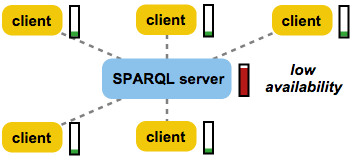
\includegraphics[width=110mm]{sparql.png}
\end{figure}



\newpage

 \begin{center}
{\fontsize{35}{35}\color{blue} \sc Problem}
\end{center}

\vspace{10 mm}

{\fontsize{30}{30} {\cmr 
\noindent {\color{blue} Hosting SPARQL endpoints requires too much effort}, both in terms of cost and server maintenance.
\\ \\
Fortunately SPARQL endpoints are not the only way of publishing queryable Linked Data.
\\ \\
\textit{Triple Pattern Fragments} is a way of publishing queryable Linked Data on low cost servers.
}} 

\newpage


\begin{center}
{\fontsize{35}{35}\color{blue} \sc LDstatic \& LDF-GAE}
\end{center}
\vspace{20 mm}
{\fontsize{30}{30} {\cmr 
\noindent We have developed two tools, LDstatic \& LDF-GAE, that implement the \textit{TPF} protocol on low cost servers.
\\ \\
{\color{blue} 
\textbf{\textit{TL;DR}}

Users can run SPARQL queries against Linked Data published on online file repositories and cloud hosting services such as \textbf{GitHub}, \textbf{Google Code}, \textbf{Google App Engine} or \textbf{Dropbox}.
}
}} 


\newpage

\begin{center}
{\fontsize{35}{35}\color{blue} \sc LDstatic}
\end{center}
\begin{figure}[ht!]


\includegraphics[width=50mm]{GitHub.jpg}
\end{figure}
\vspace{5 mm}
{\fontsize{30}{30} {\cmr 
\noindent \textbf{GitHub Pages}, and other online file repositories, can serve static HTML files.
\\ \\
It can also serve other type of content, such as N-Triples (\texttt{.nt}).
\\ \\
This means that GitHub Pages can serve triple pattern fragments.
}} 


\newpage

\begin{center}
{\fontsize{35}{35}\color{blue} \sc LDstatic}
\end{center}
\vspace{10 mm}
{\fontsize{30}{30} {\cmr 
\noindent We want to match}}
\begin{alltt}
\texttt{<foo> <bar> "literal" .}
\end{alltt}
{\fontsize{30}{30} {\cmr using:}}
\begin{alltt}
/?subject=<foo>
/?predicate=<bar>
/?object="literal"
/?subject=<foo>\&predicate=<bar>
\dots
\end{alltt}
{\fontsize{30}{30} {\cmr We need at least 8 static files for each triple if we want to match all combinations.
}} 

\newpage

\begin{center}
{\fontsize{35}{35}\color{blue} \sc LDstatic}
\end{center}
\vspace{10 mm}
{\fontsize{30}{30} {\cmr 
\noindent Having all combinations is important for triple pattern fragments enabled clients so they can run complex queries, even SPARQL queries!
\\\\
So we can host queryable linked data on GitHub Pages:
\begin{center}
\url{http://lmatteis.github.io/ldstatic/}
\end{center}
}} 



\newpage

\begin{center}
{\fontsize{35}{35}\color{blue} \sc LDF-GAE}
\end{center}
\vspace{10 mm}
\begin{figure}[ht!]
\centering

\includegraphics[width=40mm]{appengine-logo.png}
\end{figure}
{\fontsize{30}{30} {\cmr 
\noindent We now talk about our other TPF implementation, which lets us run SPARQL queries on {\color{blue}Google App Engine}.

\begin{center}
\url{http://ldf-gae.appspot.com/}
\end{center}
}} 


\newpage

\begin{center}
{\fontsize{35}{35}\color{blue} \sc LDF-GAE}
\end{center}
\vspace{20 mm}

{\fontsize{30}{30} {\cmr 
\noindent Storing triples on App Engine's high-replication datastore is quite simple. We store them using \textit{Apache Jena}'s representation.
\\ \\
{\color{blue}Stored as:}
}} 
\begin{center}
\begin{small}
\begin{verbatim}
{
  "subject"  : triple.getSubject().toString(),
  "predicate": triple.getPredicate().toString(),
  "object"   : triple.getObject().toString()
}
\end{verbatim}
\end{small}
\end{center}


\newpage

\begin{center}
{\fontsize{35}{35}\color{blue} \sc LDF-GAE}
\end{center}
\vspace{20 mm}

{\fontsize{30}{30} {\cmr 
\noindent To retrieve each triple pattern combination we use App Engine's native API calls:
}} 
\begin{center}
\begin{small}
\begin{verbatim}
// query datastore
var query = new Query('triple');
query.addFilter('subject', 
    Query.FilterOperator.EQUAL, request.getParameter('subject'));
query.addFilter('predicate', 
    Query.FilterOperator.EQUAL, request.getParameter('predicate'));
query.addFilter('object', 
    Query.FilterOperator.EQUAL, request.getParameter('object'));
\end{verbatim}
\end{small}
\end{center}


\newpage

\begin{center}
{\fontsize{35}{35}\color{blue} \sc LDF-GAE}
\end{center}
\vspace{20 mm}

{\fontsize{30}{30} {\cmr 
\noindent Here's what a request looks like:
}} 
\begin{alltt}
$curl http://ldf-gae.appspot.com/\(\hookleftarrow\)
?{\color{blue}predicate}=\(\hookleftarrow\)
http%3A%2F%2Fxmlns.com%2Ffoaf%2F0.1%2Fname
\end{alltt}
{\fontsize{30}{30} {\cmr 
\noindent \color{blue} Response:
}} 
\begin{center}
\begin{tiny}
\begin{alltt}
<http://www.kjetil.kjernsmo.net/foaf#me> {\color{blue}<http://xmlns.com/foaf/0.1/name>} "Kjetil Kjernsmo" .
<http://www.cs.umd.edu/~hendler/2003/foaf.rdf#jhendler> {\color{blue}<http://xmlns.com/foaf/0.1/name>} "Jim Hendler" .
<http://www.w3.org/People/Jacobs/contact.rdf#IanJacobs> {\color{blue}<http://xmlns.com/foaf/0.1/name>} "Ian Jacobs" .
<http://id.ecs.soton.ac.uk/person/60> {\color{blue}<http://xmlns.com/foaf/0.1/name>} "Les Carr" .
<http://people.csail.mit.edu/psz/foaf.rdf#me> {\color{blue}<http://xmlns.com/foaf/0.1/name>} "Peter Szolovits" .
<http://www.w3.org/People/EM/contact#me> {\color{blue}<http://xmlns.com/foaf/0.1/name>} "Eric Miller" .
\end{alltt}
\end{tiny}
\end{center}

\newpage

\begin{center}
{\fontsize{35}{35}\color{blue} \sc How is this novel?}
\end{center}
\vspace{20 mm}

{\fontsize{30}{30} {\cmr 
\noindent We can exploit a variety of {\color{blue}free} hosting services to publish Linked Data and have clients query them. No more sys-admin tasks. Less down times.
\\\\
For small datasets this is \textbf{more sustainable}, \textbf{more economical} and best of all it's \textbf{easier}!
}} 


\newpage

\begin{center}
{\fontsize{35}{35}\color{blue} \sc How to use?}
\end{center}
\vspace{20 mm}

{\fontsize{30}{30} {\cmr 
\noindent Both tools are on GitHub with documentation and you can use them right now: 

\url{https://github.com/lmatteis/ldstatic}

\url{https://github.com/lmatteis/ldf-gae}
}} 

\newpage

\begin{center}
{\fontsize{35}{35}\color{blue} \sc Conclusion}
\end{center}
\vspace{20 mm}

{\fontsize{30}{30} {\cmr 
\noindent We proved that triple pattern fragments is a type of linked data can be published with high availability on low-cost Web servers ranging from basic file repositories to highly scalable cloud platforms.
}} 


\newpage


\begin{center}
{\fontsize{35}{35}\color{blue} \sc References}
\end{center}
\vspace{20 mm}

{\fontsize{30}{30} {\cmr 
\noindent Linked Data Fragments --

\url{http://linkeddatafragments.org/}
\\ \\
Triple Pattern Fragments protocol -- 

\url{http://www.hydra-cg.com/spec/latest/triple-pattern-fragments/}
}} 


\newpage

\vspace*{\fill}
\begin{center}
{\fontsize{35}{35}\color{blue} \sc Thank you!}
\end{center}
\vspace*{\fill}

\end{document}